\documentclass{patmorin}
\listfiles
\usepackage{amsthm,amsmath,graphicx,wrapfig}
\usepackage{pat}

\usepackage{color}
\definecolor{linkblue}{named}{Blue}

\usepackage[letterpaper]{hyperref}
\hypersetup{
  colorlinks=true, 
  linkcolor=linkblue,  
  anchorcolor=linkblue,
  citecolor=linkblue, 
  filecolor=linkblue, 
  menucolor=linkblue, 
  pagecolor=linkblue,
  urlcolor=linkblue
} 

\DeclareMathOperator{\scc}{succ}
\DeclareMathOperator{\pred}{pred}
\DeclareMathOperator{\lft}{left}
\DeclareMathOperator{\rght}{right}
\DeclareMathOperator{\prnt}{parent}
\DeclareMathOperator{\lca}{LCA}
\DeclareMathOperator{\logsum}{logsum}
\DeclareMathOperator{\hgt}{height}

%% This code allows dynamic scaling of images to fit the page
%% Usage: \includegraphics[width=\ScaleIfNeeded]{figs/figure}
\makeatletter
\def\ScaleIfNeeded{%
\ifdim\Gin@nat@width>.97\linewidth
.97\linewidth
\else
\Gin@nat@width
\fi
}
\makeatother


\usepackage{tikz,hyphenat}
\let\oldmarginpar\marginpar
% renew the \marginpar command to draw 
% a node; it has a default setting which 
% can be overwritten
\renewcommand{\marginpar}[2][rectangle,draw,fill=yellow,rounded corners,text width=2.21cm]{%
        \oldmarginpar{%
        \tikz \node at (0,0) [#1]{#2};}%
        }
\newcommand{\note}[1]{\marginpar{\raggedright\footnotesize\nohyphens{#1}}}

\newcommand{\eps}{\varepsilon}

\title{\MakeUppercase{Dynamic Finger and Working Set: Approaching the Lower Bounds}}
\author{Luis Barba, Rolf Fagerberg and Pat Morin}


\begin{document}
\begin{titlepage}
\maketitle
%\cofeAm{0.7}{0.38}{0}{5.5cm}{3.5in}

\begin{abstract}
  This paper begins the process of making practical dynamic
  comparison-based dictionaries that have the dynamic finger and
  working-set properties.  In particular, we initiate the study of the
  exact number of comparisons needed in dynamic dictionaries that have
  these two properties.  We present a data structure with the dynamic
  finger property that performs at most $\log_2 d+o(\log d)$ comparisons
  per operation and a data structure that, for any $\eps > 0$, has the
  working-set property and performs at most $(1+\eps)\log_2 w+o(\log w)$
  comparisons per search.  Here, $d$ and $w$ are the ``finger number''
  and ``working-set number'', respectively, of the element being accessed.
  All previously-known structures with the dynamic-finger or working-set
  property perform at least $2\log_2 d$ or $4\log_2 w$ comparison,
  respectively.
\end{abstract}

\end{titlepage}

\section{Introduction}

In this paper we present comparison-based dictionaries that support
finger-search and that have the working-set property and use a
nearly-optimal number of comparisons per search.  In the remainder of
this introduction we define these terms and explain why these results
are interesting.

\subsection{Comparison-Based Dictionaries}

Comparison-based dictionaries supporting the three \emph{basic operations}
insert, delete and search represent the
classic data-structuring problem in computer science.  AVL trees, which
support all three basic operations with an asymptotically optimal running
time were discovered already in 1962 \cite{adelsson.vleski.ea:blah}.
AVL trees implement the basic operations in $O(\log n)$ time per operation
while performing at most $1.4404\log(n+2)$ comparisons between the element
being inserted/deleted/searched and the elements stored in the AVL tree.
(Here, and throughout, $\log x$ is a shorthand for $\log_2\max\{2,x\}$.)

Since the discovery of AVL trees, many other comparison-based dictionaries
have been proposed that perform at most $c\log n + O(1)$ comparison
per operation, for some constant $c>1$:  2-3 trees ($c=XX$) \cite{X},
red-black trees ($c=2$) \cite{X}, splay trees ($c=3$) \cite{X}, scapegoat
trees ($c=1+\eps$) \cite{X, Y}, skiplists ($c=e/\log e\approx XX$)
\cite{X,Y}, treaps ($c=2/\log e\approx XX$) \cite{X,Y}, and randomized
binary search trees ($c=2/\log e\approx XX$) \cite{X} are just a few of
the colorful names for data structures that support the basic operations
in $O(\log n)$ time per operation.\footnote{Some of these structures
use amortization, in which case the $O(\log n)$ running-time bound is
only an amortized bound and some use randomization, in which case the
running-time bound is an expected running time bound, with the expectation
being taken over random choices made within the data structure.}

A handful of lesser-known structures reduce the constant $c$ to 1 while
still supporting all operations in $O(\log n)$ time: Lai, Andersson, and
Fagerberg \cite{X,Y,Z} each present data structures supporting each of
the basic operations in $O(\log n)$ (amortized) time using at most $\log
n + O(1)$ comparisons.  Since $\log(n+1)$ is an information-theoretic
lower-bound on the \emph{expected} number of comparisons when searching
for a random key, these results more or less close book on the worst-case
number of comparisons achievable by comparison-based dictionaries that
support all operations in $O(\log n)$ time.


%For these structures, the goal is to minimize the number of comparisons
%while still supporting all operations in $O(\log n)$ time.  In their
%theses \cite{X,Y} and in resulting papers, Lai and Andersson \cite{X,Y,Z}
%present a series of schemes for maintaining binary search trees with
%height at most $\lceil\log(n+1)\rceil+1$ in $O(\log n)$ time per insert,
%update, and remove operation.  Note that $\lceil\log(n+1)\rceil$ is
%a lower-bound on the height of any binary search tree containing $n$
%elements, so these trees are within 1 of the minimum possible height.

%Fagerberg \cite{fagerberg:complexity} tightens these results even
%further by showing that, for any $c>0$, it is possible to maintain
%a binary search tree with height at most $\lceil\log(n+1)+c/\log
%n\rceil$ while still performing all operations in $O((1/c)\log n)$
%amortized time.  This result is matched by a lower-bound: No binary
%search tree that performs insertions and deletions in $O((1/c)\log n)$
%time can guarantee a height smaller than $\lceil\log(n+1)+c/\log n\rceil$
%\cite{fagerberg:binary-how-low-can-you-go}.  Taken together, this upper
%bound and lower bound more or less close the book on the worst-case
%number of comparisons achievable by comparison-based dictionaries that
%support all operations in $O(\log n)$.

\subsection{Dictionaries with Properties}

A more recent trend in the design of comparison-based dictionaries is the
study of dictionaries with special running-time \emph{properties}.  These
results are motivated by a practical observation: in real applications,
queries are usually not independently and uniformly distributed, so the
information-theoretic lower bound does not apply.  Data structures having
properties that exploit special patterns in query sequences do better than
$\Theta(\log n)$ time per query.  Examples of such properties include:
\begin{description}
\item[the static-optimality property:] in which the average access time is
    proportional to the (empirical) entropy of the distribution of
    searches.  

    The study of \emph{biased dictionaries}, that satisfy the
    static-optimality property has a long and rich history.  It is
    known that, given a set of keys and a distribution of queries,
    it is possible to construct, in quadratic time, a binary search
    tree that minimizes the expected number of comparison per search
    \cite{knuth}.  A nearly optimal binary search tree, that does at
    most two extra comparisons per search can even be constructed in
    linear time \cite{mehlhorn}.

\item[the dynamic finger property:] in which the time to perform the
    current search for an element, $x$, is logarithmic in the difference,
    $d$, in ranks between the element $x$ being searched for and the
    element, $x_0$, returned as a result of the previous search. (During
    the first access, $d$ is defined to be $n$.)

    Several data structures are known that can perform searches
    in $O(\log d)$ time using $c\log d+o(\log d)$ comparisons; these
    include homogeneous finger search trees ($c=4$) \cite{tarjan:xxx},
    splay trees ($c=250,000$) \cite{cole} treaps ($c=4/\log e$)
    \cite{sksk}, and skiplists  ($c=2e/\log e$) \cite{sksk}, and
    unary-binary trees augmented with hands ($c=2$) \cite{X,Y}.
    See Brodal \cite{brodal:finger} for a recent survey on finger search.

\item[the working-set property:] in which the time to perform the current
    search for an element, $x$, is logarithmic in the number, $w$, of
    distinct elements accessed since the most recent previous access to
    $x$.  (If this is the first access to $x$, then $w$ is defined to be $n$.)

    Several data structures are known that can perform searches in
    $O(\log w)$ time using $c\log w+o(\log w)$ comparisons; these include
    splay trees ($c=4$) \cite{X},\footnote{Tarjan and Sleator's Working
    Set Lemma \cite{X} gives the bound $c=8$.  However changing their
    potential from $1/w(i)^2$ to $1/w(i)\log^2 w(i)$ improves this to
    $c=4$.} several variants of Iacono's doubly-exponential structure
    ($c\ge 4$) \cite{X}, variants of skiplists and B-trees ($c=??$),
    and layered working-set trees ($c=??$) \cite{hXX}.

    It is worth noting that the working-set property is stronger than the
    static optimality property.  Roughly speaking, any data structure
    that has the working-set property with constant $c$ can perform a
    sufficiently long sequence of searches with an average of $c\tilde{H}$
    comparisons per search, where $\tilde{H}$ is the empirical entropy of
    the search sequence \cite{X,Y}.  Note that, unlike the results for
    static optimality, this does not require advanced knowledge of the
    query distribution.  This observation, which follows from Jensen's
    Inequality, is the basis of one of the most effective and practical
    data compression algorithms known \cite{mtf-compression,bzip}.

\end{description}
Additional properties have been proposed, including the unified property
\cite{IXX} and the dynamic optimality property \cite{X}, but the three
properties discussed above are among the oldesseem to be among the most fundamental.

%A classic
%result in this area is that of Mehlhorn \cite{mehlhorn:best}.
%Mehlhorn's algorithm takes as input a probability distribution
%$q_0,p_1,q_1,p_2,q_2,\ldots,p_n,q_n$ and a sequence of keys
%$x_0=-\infty<x_1<x_2<\cdots<x_n<x_{n+1}=\infty$.  Each $p_i$
%represents the probability of searching for the key $x_i$ and $q_i$
%represents the probability of searching for a key in the open interval
%$(x_{i},x_{i+1})$. Mehlhorn's algorithm then builds, in linear time,
%a binary search tree containing $x_1,\ldots,x_n$ where the depth of
%$x_i$ is at most $\log (1/p_i)+1$ and the length of the search path
%for any element in the interval $(x_i,x_{i+1})$ is at most $\log
%(1/q_i)+2$. With the exception of the additive constants, 1 and 2,
%these bounds are essentially the best-possible.  

\subsection{Constants for Dynamic-Finger and Working-Set}

Unfortunately, dictionaries with properties generally fail to deliver on
the practical results they promise, and this is due to the constants in
their running times.  To illustrate this, consider a binary search tree,
$T$, that contains $n=10^6$ elements, and is implemented using Andersson,
Lai, or Fagerberg's binary search trees.  Such a structure can perform
any search using at most
\[
   \lceil\log(10^6+1)\rceil+1= 21
\]
comparisons.  In contrast, consider storing the same elements in a
dictionary, $S$, implemented using splay trees.  The (amortized) number
of comparisons performed during a search in $S$ is $4\log w+o(\log w)$
(see \secref{working-set}).  Thus, in order for $S$ (a splay tree)
to perform faster than $T$ (a balanced binary search tree), we must have
\[
   4\log w < 21 
       \Leftrightarrow \log w < 5.25 
       \Leftrightarrow w \le 38 \enspace .
\]
That is, of the one million elements stored in $S$ and $T$, there are only
38 that can be accessed faster in $S$ than in $T$.  Most of the remaining
$10^6 - 38$ elements require more comparison to access in $S$ than in $T$,
and the vast majority require a factor of 2--4 times as many comparisons.

To further widen the performance gap, the splay tree, $S$, performs
$3\log w$ rotations after every search, while searches do not affect
the structure of $T$ at all.  Taking all this into consideration,
it seems difficult to imagine \emph{any} realistic application where
the working-set property of splay trees would give better performance
than (Andersson, Lai, or Fagerberg's) balanced binary search trees.
(This back-of-the- envelope analysis is born out by several experimental
evaluations of splay trees \cite{X,X,X}.)

\subsection{New Results}

So it seems that a necessary condition for a dynamic-finger structure
or a working-set structure to be practical is that the leading constant
on the number of comparisons performed during a operation should be very
small; ideally this constant should be 1.  In this paper we present two
data structures that attempt to achieve this ideal.  Our first data
structure supports dynamic-finger operations in $O(\log d)$ time and
performs at most $\log d+o(\log d)$ comparisons during any operation. Our
second data structure is parameterized by a parameter $\eps >0$ and
supports all operations in $O(\eps^{-1}\log w)$ time and performs
at most $(1+\eps)\log w+o(\log w)$ comparisons during any operation.
(Note that $\eps$ may even depend on $n$.)

\subsection{Focusing on Comparisons}

We do not claim that minimizing comparisons immediately implies that our
data structures are efficient in practice. Like all dictionaries, our
algorithms perform operations other than comparisons, so justifying such a
claim would require some algorithms engineering to streamline and tune our
data structures as well as a rigorous experimental evaluation.  Our only
claim is that our data structures satisfy a necessary condition that
prevents existing structures, such as splay trees, from being practical.

Nevertheless there are programming environments that tilt the table
heavily towards the goal of minimizing comparisons.  Consider, for
example, the Java Collections Framework \cite{jcf}.  In the JCF,
a single comparison between two \texttt{Integer} objects stored in a
\texttt{SortedMap} (which is implemented as a red-black tree) involves
\begin{enumerate}
  \item dereferencing the data structure's \texttt{Comparator} object,
    \texttt{c} (\texttt{this.c});
  \item calling \texttt{c}'s \text{compare(a,b)} method, which requires
    both a function call and a dereferencing operation in \texttt{c}'s
    dispatch table (\texttt{c.compare(a,b)}); and
  \item the \texttt{compare(a,b)} method must then dereference \texttt{a}
    and \texttt{b}'s native \texttt{int} variables and compare
    them by computing their difference using the \text{isub}
    instruction. (\texttt{return a.value - b.value})\footnote{In Java,
    the \texttt{compare(a,b)} method should return a negative value if
    $\mathtt{a} < \mathtt{b}$, zero if $\mathtt{a} = \mathtt{b}$ and a
    positive value if $\mathtt{a} > \mathtt{b}$.}
\end{enumerate}
In this way, a single comparison performed within the data structure
involves a function call and four dereferencing operations, each of
which is an order of magnitude slower than the \texttt{isub} instruction
that actually performs the comparison.  One could argue that this
is a(nother) reason not to develop performance-critical software in
Java, but given that there are already 3 billion devices running Java
\cite{www.java.com/en/about}, it is still a worthwhile goal to optimize
algorithms for it.

%\section{Background}
%
%\subsection{Bentley and Yao's unbounded Search.}
%
%\subsection{Unbounded Search}
%
%\begin{thm}\thmlabel{unbounded-search}
%After this, one can use a straightforward modification of Bentley
%and Yao's unbounded search algorithm \cite{byXX,kXX,xxx} to find $x$
%at some position $a_j$ in $\log w + O(\log\log w)$ comparisons, where
%$w=|i-j|$.\footnote{Bentley and Yao actually prove the somewhat stronger
%result that the number of comparisons required is at most $\log w +
%\log\log w + \log\log\log w +\cdots + O(\log^* w)$.  See also, Knuth
%\cite{kXX} and Beigel \cite{bXX}.}
%\end{thm}
%
%\subsection{Fagerberg's 1-2 Trees}
%
%Fagerberg's 1-2 trees \cite{fagerberg:complexity}, maintain a 1-2 tree
%of height at most $\log n +O(1)$, support insertion and deletion, and
%have an amortized rebalancing cost of $O(1)$ per update.  We modify this
%data structure slightly so that all keys are stored in the leaves. Each
%internal node, $u$, stores a value that upper-bounds the largest value
%stored at any leaf in $u$'s subtree. However, this value never exceeds the
%smallest value stored in any leaf to the right of $u$'s subtree\ldots
%
%Mention that a node of height $h$ has $2^{h-O(1)}$ leaf descendants.
%
%


\section{The Dynamic-Finger Property}

Other than splay trees (which have an enormous constant), data structures
that perform finger search typically work in two phases.\footnote{Even
splay trees can be viewed as having a two-phase approach to finger search;
the first phase (splaying) takes place while searching for the previous
element).} In the \emph{upward phase} the search starts at the current
node, which contains $x_0$, and walks upwards in the data structure
until reaching a node, $w$, from which the usual search procedure can
be applied.  In the \emph{downward phase} a search for $x$ that starts
at $w$ is performed.

This two phase approach is expensive: If the worst-case number of
comparisons done during a (non-finger) search is $c\log n+o(\log n)$ the
two phase approach usually leads to a search time of $2c\log d+o(\log d)$;
using a simple two-phase finger search on a normal structure doubles the
leading constant.  Informally, this is because the logarithm is such a
slow-growing function: If $w$ is a node containing a value equidistant
from $x_0$ and $x$, then the the number of comparison used to go from
$x_0$ to $w$ and then to $x$ is $c\log(d/2) + c\log(d/2) = 2c\log d - 2c$.
This is the reason no existing structure has a constant smaller than 2.

We note that there are several approaches to resolve this problem.
One particularly easy method is to modify the upward phase of a two
phase algorithm so that it only performs $O(\log \log d)$ comparisons.
This modification involves a straightforward implementation of exponential
search (discussed below).  In typical existing structures, all of
which are pointer based, this modification will decrease the number of
comparisons during the upward phase, but the running time will still
be $O(\log d)$.  (This is analogous to implementing binary search on a
linked list; the number of comparisons is logarithmic, but the running
time is still linear.)

\subsection{Overview}

We will describe two phase approach to finger search in which the
first phase runs in $O(\log\log d)$ time and performs $O(\log\log d)$
comparisons and the second phase runs in $O(\log d)$ time and performs
$\log d+ O(1)$ comparisons.

At a high level, our new structure works as follows: We use an extremely
well-balanced search tree, $T$, which has height $\log n+ O(1)$.
We then use an auxiliary structure of size $O(\log n)$ that keeps track
of information about the search paths around $x_0$.  This structure is
an array-based variant of Blelloch \etal's \emph{hands} data structure.
Our version of hands supports two phase finger searches with the first phase
running in $O(\log\log d)$ time and the second phase running in $O(\log
d)$ time.

Of course, there is an issue with this approach that needs to be resolved.
Blelloch \etal's hands are a pointer-based structure that make use of
the fact that linked lists can be split and joined in constant time.
To obtain our speedup of the first phase, we require an array-based
structure.  This is a problem since, in general, arrays can not be split
and joined in constant-time.  We show that this problem can be handled
effectively using an indexing trick.  As a side-effect, we obtain
an array-based version of Blelloch \etal's hands that is (arguably) easier
to maintain and likely to be more efficient than the original version.

\subsection{Tools}

We begin with a short discussion of the three tools used by our algorithm.

\subsubsection{Unbounded Search in a Sorted Array}

A standard method for searching in a sorted array, $A=a_1,\ldots,a_n$,
when there is reason to believe that the search result is closer to
the front of the array than the back is \emph{exponential search}.
To find the position of some query value, $x$, we examine $a_1$,
$a_2$, $a_4$, $a_8$, and so on until finding the first value, $j\ge 0$,
such that $a_{2^j} \ge x$.  At this point, a standard binary search
over $a_{2^{j-1}}+1,\ldots,a_{2^j}$ can be used to find $x$ using an
additional $j$ comparisons.

Exponential search uses $2j$ comparisons. On the other hand, the index,
$i$, of $x$, is greater than $2^{j-1}+1$, so the number of comparisons
performed by exponential search, when the search result is at position
$i$, is at most $2\lceil\log i\rceil\le 2\log i + 1$.  The idea behind
exponential search has been refined by Bentley and Yao \cite{byXX}.
Using their algorithm one can, for example, find $x$ using $\log i+
O(\log\log i)$ comparisons.

%
%.  Define the \emph{iterated logarithm function}
%\[
%    \log^{(j)} x = \begin{cases}
%       x & \text{if $j=0$} \\
%       \log(\log^{(j-1)} x) & \text{if $j>0$}
%    \end{cases}
%\]
%and define $\log^* x=\min\{j: \log^{(j)} x \le 1\}$.  The following result,
%due to Bentley and Yao \cite{bentley.yao.XX} is a generalization of
%exponential search \cite{X}:
%
%\begin{thm}[Bentley and Yao]\thmlabel{bentley-yao}
%There exists an algorithm that takes as input a sorted array,
%$A=a_1,\ldots,a_n$, and a value, $x$, and finds the smallest index, $i$,
%such that $a_i\ge x$ or returns $n+1$ if $x>a_n$.  This algorithm runs
%in $O(\log i)$ time and performs
%\[
%    \logsum(i) = \sum_{j=1}^{\log^* i} \log^{(j)} i + O(\log^* i)
%\]
%comparisons.
%\end{thm}
%
%We observing that \thmref{bentley-yao} makes it easy to obtain a
%static dictionary---one that does not support the insert or delete
%operations---that has very fast finger search.  Simply store the data in
%a sorted array, $A=a_1,\ldots,a_n$, and maintain the index, $i$, of the
%most recently accessed element, $x_0$.  When it comes time to search
%for the next element, $x$, a single comparison between $x$ and $x_0$
%suffices to determine if the search should proceed in $a_i,\ldots, a_n$
%or in $a_{i-1},\ldots,a_1$ after which one can apply \thmref{bentley-yao}
%to find $x$ in $O(\log d)$ time using $\logsum(d)=\log d + O(\log\log d)$ comparison.
%

\subsubsection{1-2 Trees}

To obtain a dynamic dictionary, we will use a special kind of very well
balanced binary search trees.  A \emph{unary-binary tree} or \emph{1-2
tree} is a tree in which all the leaves have the same depth and every
internal node has one (a unary node) or two (a binary node) children.
The following result, due to Fagerberg \cite{X}, is used in the
maintenance of binary trees of very low height:

\begin{thm}[Fagerberg]
  It is possible to maintain a unary-binary search tree, $T$, under the
  operations of insertion and removal in constant amortized time per
  operation so that, after every operation
  \begin{enumerate}
    \item(low height) $T$ has height $\log n + O(1)$, where $n$ is the
      number of leaves currently in the tree;
    \item(exponential size) every node of height $h$ is the root of a
      subtree having at least $c2^h$ leaves, for some constant $c>0$; and
    \item(no adjacent unary) the child of each unary node is either 
      a leaf or a binary node.
   \end{enumerate}
\end{thm}

\subsubsection{Hands}

Blelloch \etal\ introduce a data structure, that they call ``hands''
that augments a degree-balanced search so that it supports efficient
finger search.  Hands consist of four lists.  The first two of these lists
are called $L$ and $R$.  Suppose the most recently accessed value was
$x_0$. To understand the contents of $L$ and $R$, consider the standard
drawing of a binary search tree, where the $x$ coordinate of each node
is given by its key and the $y$-coordinate is given by its height.
If we draw a vertical line through $x_0$, then $L$ contains those nodes
immediately to the left of (and on) this line and $R$ contains those nodes
immediately to the right of (and on) this line (see \figref{search-path}).
(Informally, $L$ and $R$ contain the search paths for $x_0-\epsilon$ and
$x_0+\epsilon$.)  The nodes on these paths are ordered from bottom-to-top,
so that $L[i]$ and $R[i]$ are nodes of height $i$.

\begin{figure}
  \begin{center}
    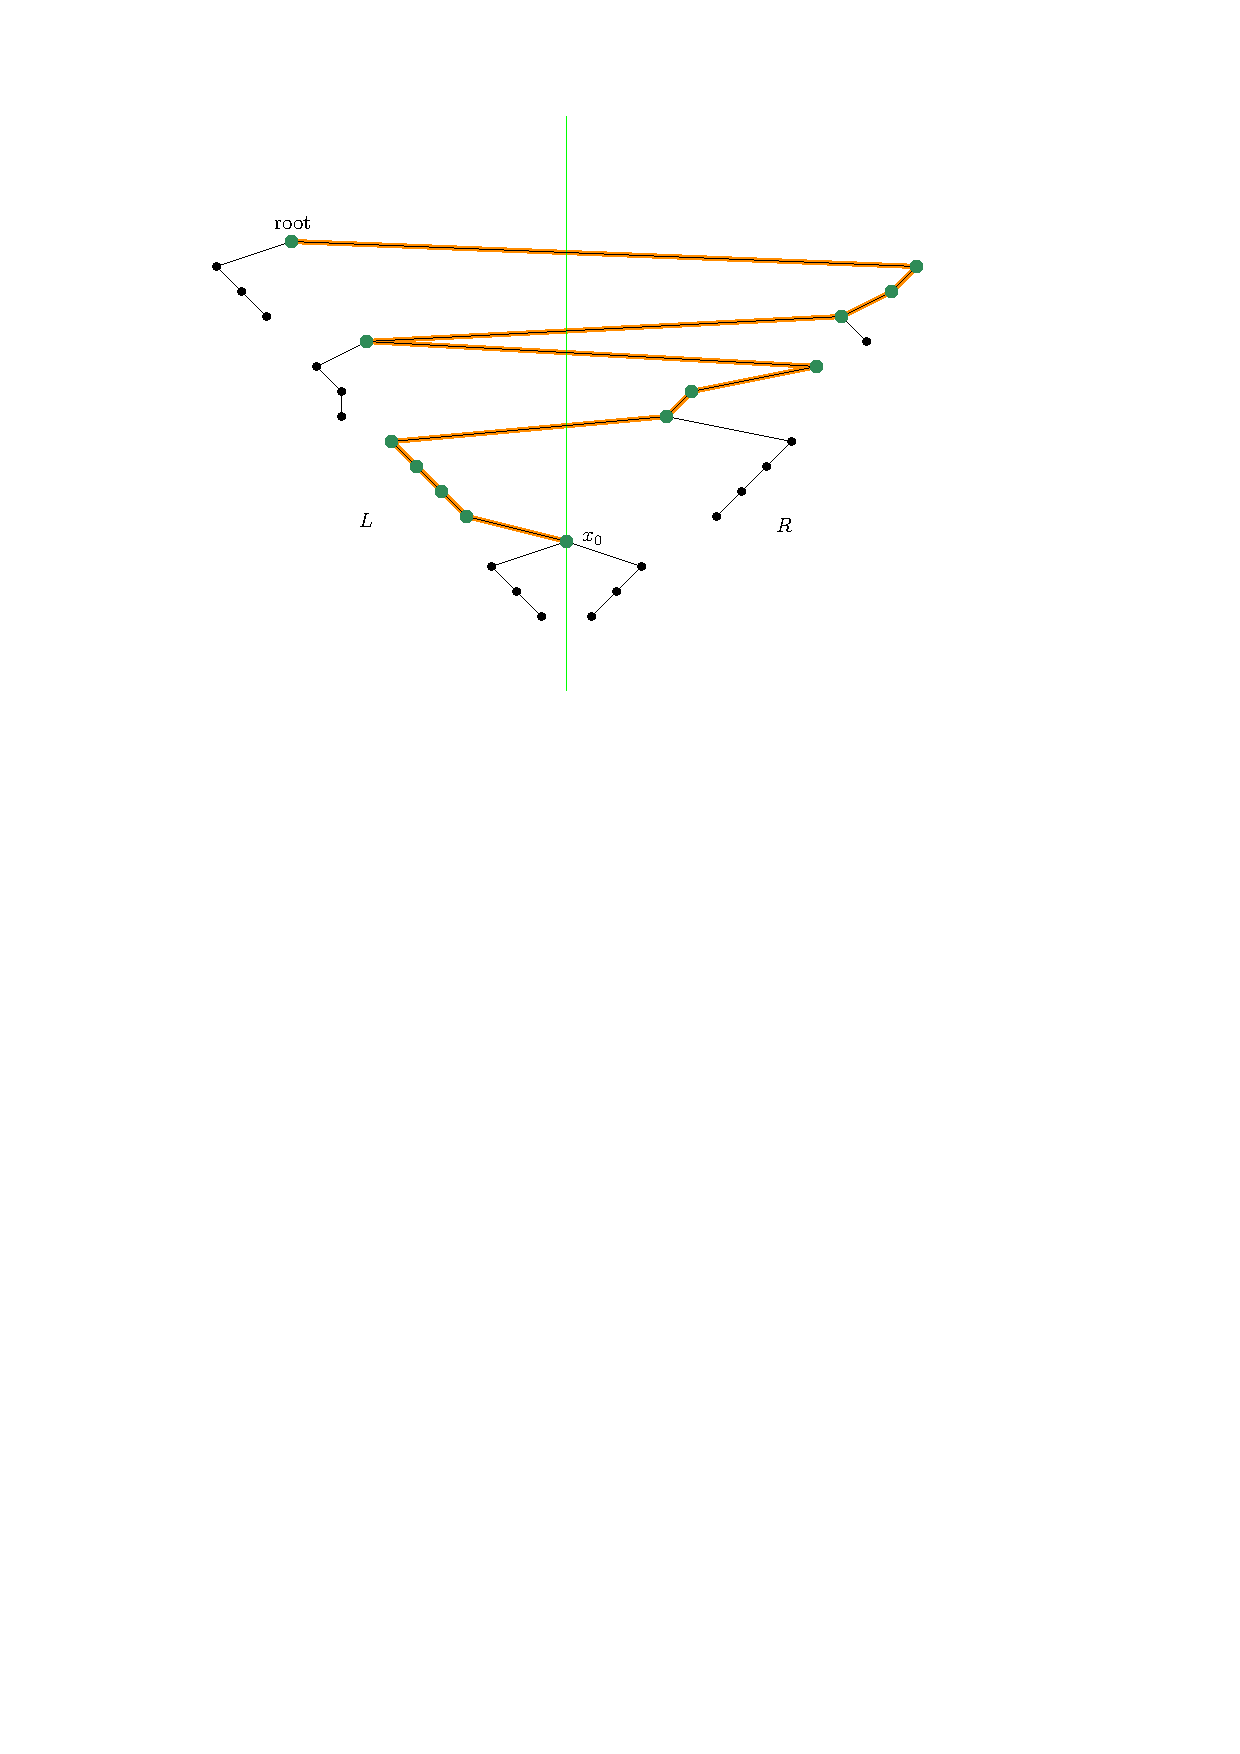
\includegraphics[width=\ScaleIfNeeded]{search-path}
  \end{center}
  \caption{Blelloch \etal's hands: The search path for $x_0$ is in orange. Every node is contained in $L$ and/or $R$.  The stacks $L^+$ and $R^+$ contain the large green nodes.}
  \figlabel{search-path}
\end{figure}

In addition to the two lists $L$ and $R$, two stacks, $L^+$ and $R^+$,
also implemented as lists, are maintained. $L^+$ contains those nodes
on the search path for $x_0$ that are less than or equal to $x_0$ and
$R^+$ contains those nodes that are greater than or equal to $x_0$.
These stacks are ordered so that the nodes closer to $x_0$ are closer
to the top of the stack and $x_0$ itself is the top element on each the
stack. Note that the elements of $L^+$ and $R^+$ are a subset of those
in $L$ and $R$, respectively.

\paragraph{Finger Search.}
Refer to \figref{hand-search}.
Suppose, without loss of generality, that we want to perform a search for
some value $x>x_0$.  To do this, we repeatedly examine the top element
of $R^+$ and pop it off if it is less than $x$.  This process pops off
at least one element, since $x_0<x$.  Consider the last element $\hat
x$ popped off the stack.  It must be the case that $x=\hat x$ or $x$
is in the right subtree of $\hat x$.  Unfortunately, searching in $\hat
x$'s subtree may be too slow; the height of this subtree has no relation
to $d$.

\begin{figure}
  \begin{center}
    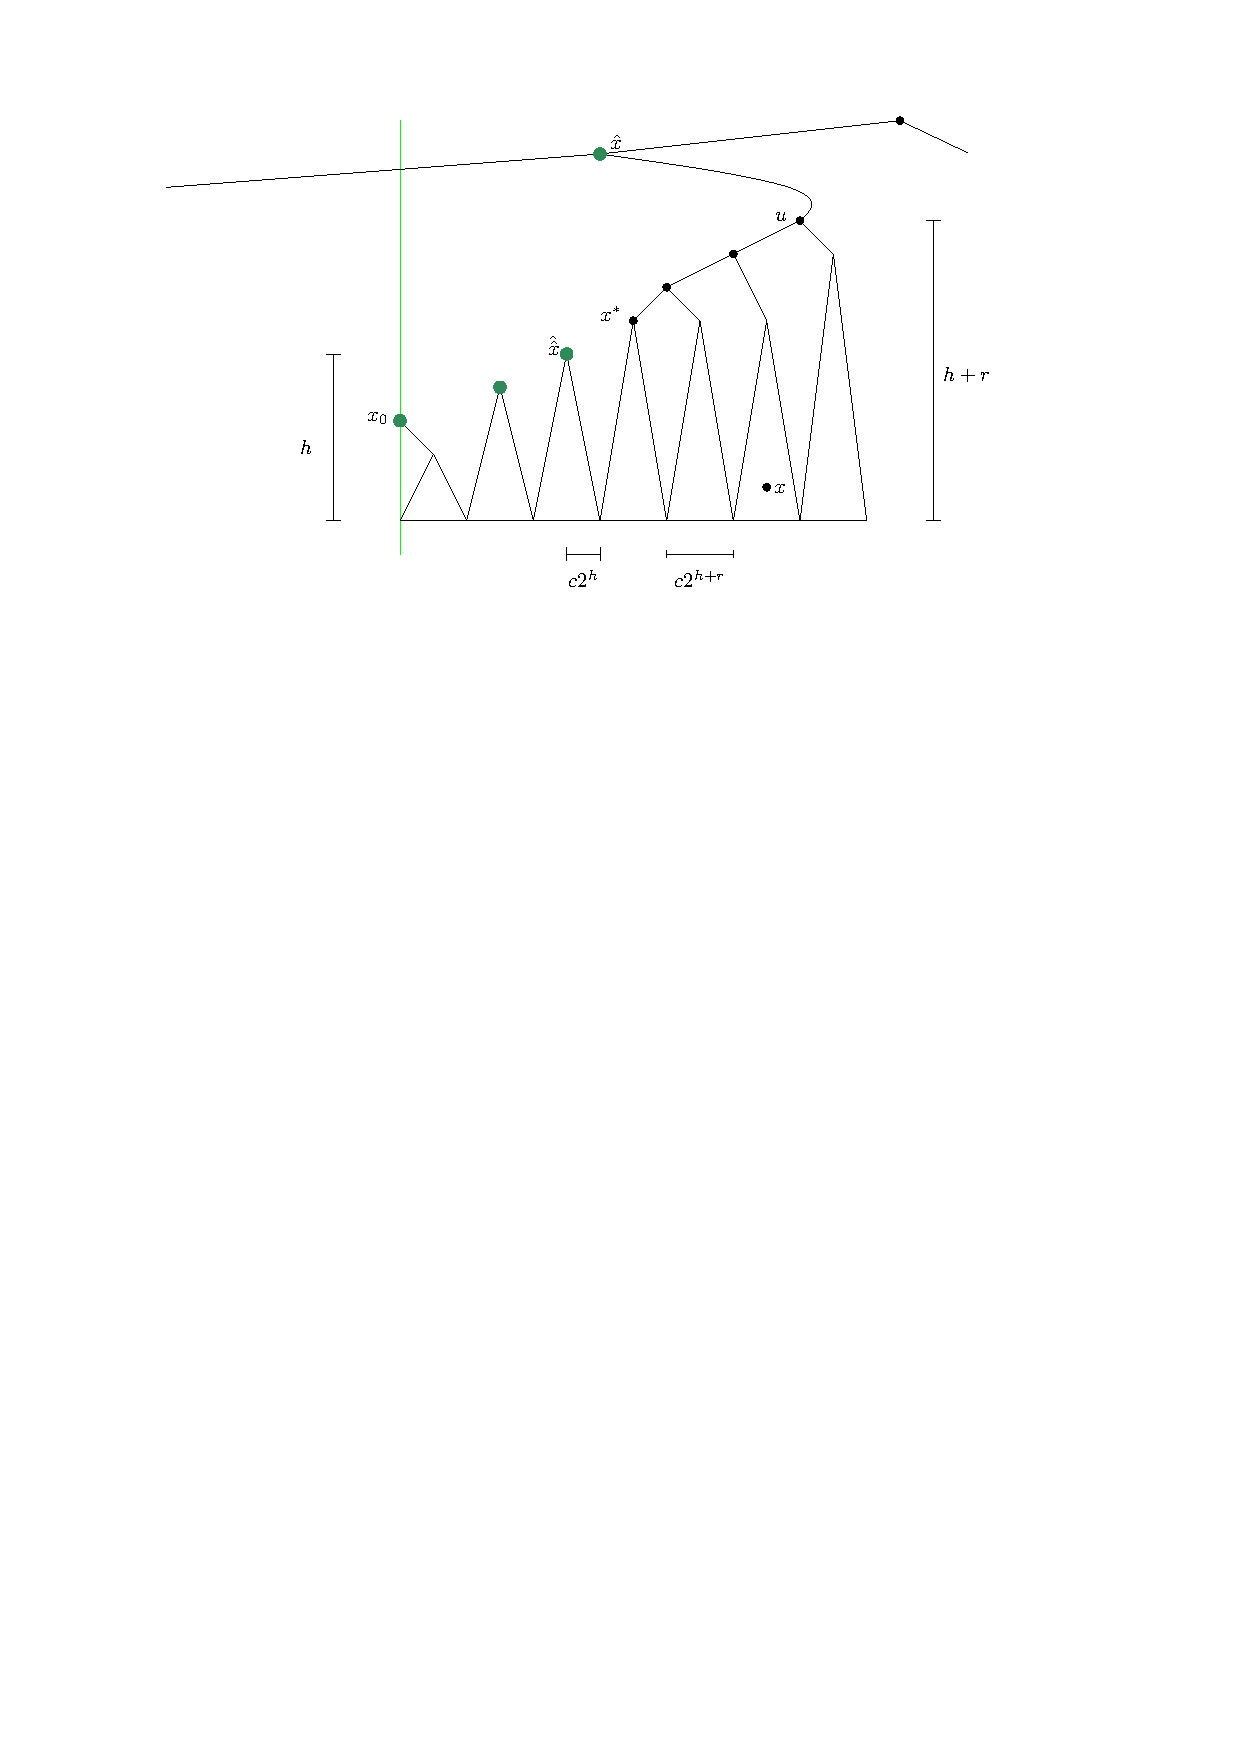
\includegraphics[width=\ScaleIfNeeded]{hand-search}
  \end{center}
  \caption{Performing a finger search using a hand.}
  \figlabel{hand-search}
\end{figure}

Consider the second-last element of $\hat{\hat x}$ that was popped
off the stack (if no such element exists, imagine $\hat{\hat x}$ is
the external node, of height $-1$, that is just to the right of $x_0$).
Now, $\hat{\hat x}$ has some height, $h$, and therefore $\hat{\hat x}$'s
right subtree has size at least $c2^h$.  All the elements in $\hat{\hat
x}$'s right subtree are in the interval $(x_0,x)$, so $d\ge c2^h$.
In other words, we can afford to spend $O(h)$ time to find $x$.

The list $R$ contains $\hat{\hat x}$ as well as a vertex $x^*$ that is one
level above $\hat{\hat x}$.  The vertex $x^*$ is either equal to $\hat
x$ or is in $\hat x$'s right subtree.  By starting at $x^*$ and walking
upwards until reaching a node whose value is greater than $x$, we find
a node, $u$, of height $h+r$ that is an ancestor of the node $x$ we are
searching for.  Since $u$ is the first such node, we also know that $d >
c2^{h+r-1}$, so we can afford to search for $x$ starting from node $u$.

\paragraph{Updating the Hands.}
In this way, we find $x$ in $O(h+r)$ time using at most $2(h+r)$
comparisons.  What remains is to update $L$, $R$, $L^+$, and $R^+$.
One can observe that $L$ and $R$ only change at indices $0,\ldots,h+r$
and updating $L[0],\ldots,L[h+r]$ and $R[0],\ldots,R[h+r]$ is easy to
do in $O(h+r)$ time starting from the node $u$.

The tricky part is updating $L^+$ and $R^+$.  Updating $L^+$ is the
easier of the two.  It is first truncated so that it doesn't contain
any nodes at height lower than the height of $\hat x$ (Blelloch \etal\
manage this by maintaining cross pointers between elements of $L$ and
$R$ at the same level as well as cross pointers between elements of $L$
and $L^+$ and $R$ and $R^+$). The stack $L^+$ is then extended by adding
the appropriate nodes on the search path from $u$ to $x$.

To update $R^+$ Blelloch \etal\ make use of the fact that lists are
concatenable. The sequence of nodes that need to be added to $R^+$
are those on the search path from $\hat x$ to $x$.  The portion
of this path from $\hat x$ to $u$ can be spliced from the sublist
$R[h+r],\ldots,R[\hgt(\hat{x})]$. The portion from $u$ to $x$ can be
added to $R^+$ while performing the search from $u$ to $x$.

\subsection{Fast Hands}

To speed up Blelloch \etal's hands, we implement the lists $L$ and $R$
as arrays.  The lists $L^+$ and $R^+$ are also implemented as arrays,
but not in the obvious way.  Recall that $L^+$ and $R^+$ store nodes
on the search path for $x_0$, and these nodes are also stored in $L$
and $R$, respectively.

Observe that the search path for $x_0$ alternately takes subpaths of
$L$ and subpaths of $R$.  Therefore, we can represent $L^+$ and $R^+$
as a sequence of pairs of indices, where the pair $(\ell,h)$ in, for
example, $R^+$ indicates that the stack represented by $R^+$ contains the
elements $R[\ell],\ldots,R[h]$.  We can even implement $R^+$ and $L^+$
as a single array, with odd indices for $R^+$ and even indices for $L^+$;
this combined array then represents the entire search path for $x_0$. See
\figref{fast-hand.xml}.

\begin{figure}
  \begin{center}
    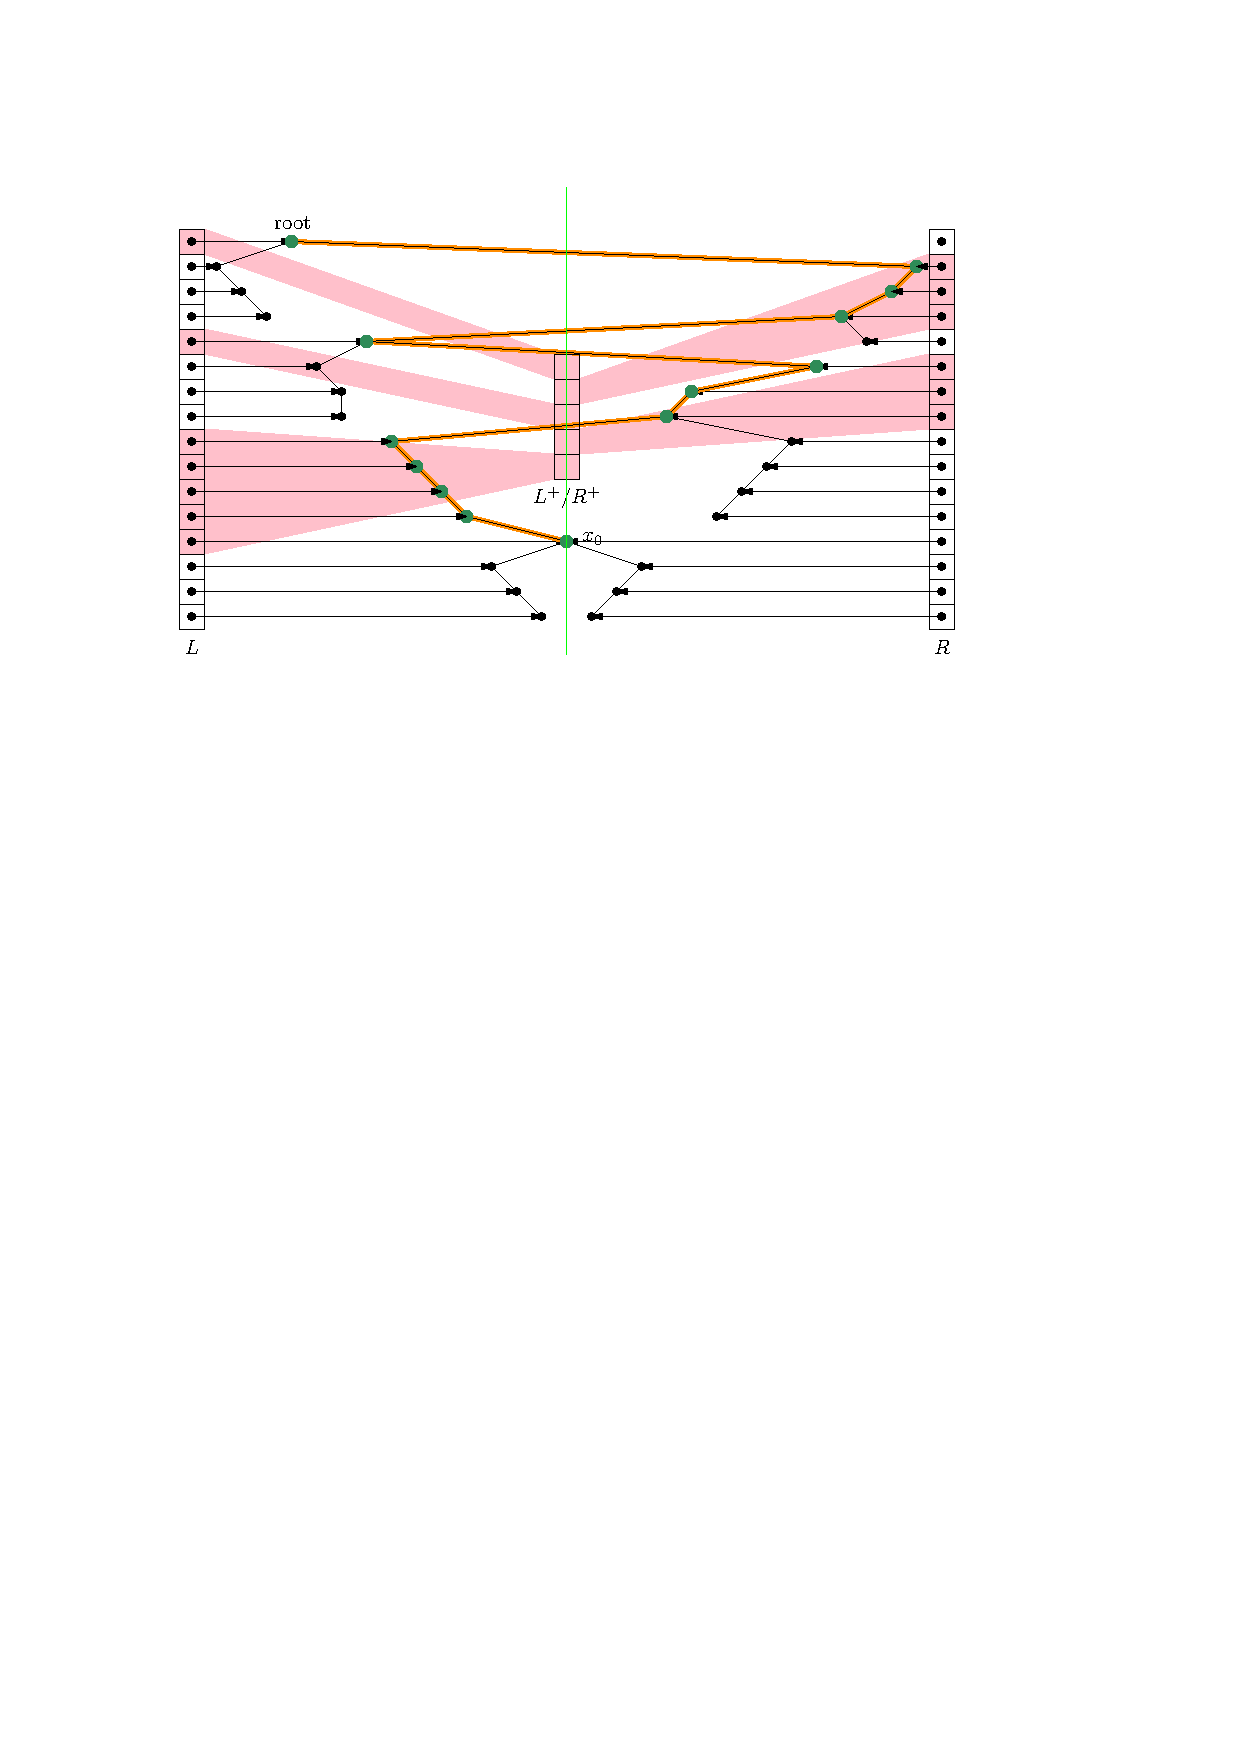
\includegraphics[width=\ScaleIfNeeded]{fast-hand}
  \end{center}
  \caption{An array-based implementation of hands.}
  \figlabel{fast-hand}
\end{figure}

We will use the notation $R^+_{[]}$ and $L^+_{[]}$ to denote the array
of pairs that represents the stack $R^+$ and $L^+$, respectively.
We observe that this representation of $R^+$ and $L^+$ still allows
for exponential search.  To perform a search on $R^+$, for example, we
perform exponential search on $R^+_{[]}$ to find an interval $(\ell,
h)$ that contains the element we are searching for.  We then perform
exponential search, within $L$ and starting at position $\ell$, to find
the element in $L$ that we are searching for.  If the element we are
searching for is at distance $i$ from the top of the stack $R^+$, then
it is straightforward to verify that double application of exponential
search takes $O(\log i)$ time and performs $O(\log i)$ comparisons.

\paragraph{Finger Search.}

Recall that a finger search for $x>x_0$ first searches $R^+$ in order
to find $\hat x$ and then searches $R$ in order to find $u$.  In our
array-based representation, the first of these searches can be done in
$O(\log h)$ time and the second search can be done in $O(\log r)$
time using exponential search.  Since $d\ge c2^{h+r}$, this implies that
the upward phase of the algorithm that $O(\log\log d)$.

\paragraph{Updating the Hands.}

Updating $L$ and $R$ during a finger search is easy.  These arrays only
need to be updated at positions $0,\ldots,h+r$ and this can be done
starting $u$, in $O(h+r)$ time (see Blelloch \etal\ \cite{x} for details).

To update $L^+$, we first need to truncate it so that it does not
contain any nodes lower than hand $\hat x$.  Note that we have located
$\hat x$ in $R^+_{[]}$.  In particular, we have found an index $i$
such that $R^+_{[]}[i]$ is an interval of $R^+$ that contains $\hat x$.
This means we want to truncate $L^+$ at location $i$ or $i+1$, so this
can be done in constant time.  The only other update required on $L^+$
is to add nodes on the search path from $u$ to $x$, which can be done
while traversing this path.

To update $R^+$ we first truncate $R^+$ at $\hat x$, which is easily
done in constant time, since we have already located the interval of
$R^+_{[]}$ that contains $\hat x$. Next, we need to add the path from the
right child of $\hat x$ to $u$.  This can also be done in constant time
by appending the pair $(h+r,\hgt(\hat x)-1$ to $R^+_{[]}$.  Finally,
we add the appropriate elements on the search path from $u$ to $x$
while traversing this path.

In summary, it is possible to perform a finger search and update the
hands in $O(\log d)$ time using $\log d+O(\log\log d)$ comparisons.

\paragraph{Insertion and Deletion.} 1-2 trees support insertion and
deletion in constant amortized time provided that a pointer to the node
being deleted or a pointer to the location of the insertion is given.
The appropriate pointer is easily obtained using finger search.

During an insertion of deletion, the 1-2 tree is modified.  Updating the
hands during these modification can be done in time proportional to the
number of modifications (see Blelloch \etal\ for details).   Therefore,
updating the hand does not increase the asymptotical running-time of
insertions or deletions.  The following theorem summarizes our result
for finger search

\begin{thm}
  There exists a linear-sized comparison-based dictionary that
  supports searching in $O(\log d)$ worst-case time using at most $\log
  d+O(\log\log d)$ comparisons.  Insertions and deletions in this data
  structure involve a single search plus a constant amortized amount of
  restructuring that can be done in constant amortized time.
\end{thm}

Finally, it is worth noting that our structure maintains all the
advantages of hands: It has only $O(\log n)$ size; it does not require
any special augmentation (such as level links) of the underlying search
tree $T$, and several processes can share the same search tree, $T$,
each maintaining its own hand.  For binary search tree fetishists, this
structure can even be implemented as a binary search tree by collapsing
unary nodes (see Fagerberg \cite{fXX} for details).


\section{The Working-Set Property}

Our working set data structure is a variant of a skiplist.  It consists of a sequence of lists $L_0,\ldots,L_k$ where
\begin{enumerate}
  \item $|L_0|\in O(1)$
  \item every element in $L_i$ appears in $L_{i+1}$ for all
  $i\in\{0,\ldots,k-1\}$;
  \item $L_i$ contains every element, $x$, such that $w(x)\le (2-\epsilon)^i$;
  \item if $x$ and $y$ are two consecutive elements of $L_i$, then at
  least one of $x$ and $y$ appears in $L_{i-1}$.
\end{enumerate}

\subsection{Searching}

A search in a

\section{Discussion}

\subsection{Two-Way Comparisons}

\subsection{Handling Searches for Missing Values}

\section*{Acknowledgement}

The authors of this paper are partly funded by NSERC and CFI.

\bibliographystyle{abbrvurl}
\bibliography{fastws}

\newpage

\section*{Authors}

\noindent
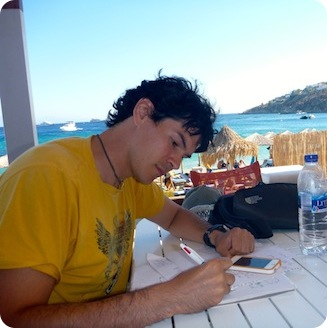
\includegraphics[width=.3\textwidth]{luis-b}% 
\hspace{.05\textwidth}%

\includegraphics[width=.3\textwidth]{rolf-b}% 
\hspace{.05\textwidth}%
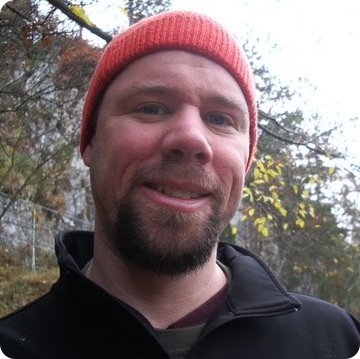
\includegraphics[width=.3\textwidth]{pat-b}%

\noindent\emph{Luis Barba.}
D\'epartement D'Informatique, Universit\'e Libre de Bruxelles
and
School of Computer Science, Carleton University

\noindent\emph{Rolf Fagerberg.}
Department of Mathematics and Computer Science, University of Southern Denmark

\noindent\emph{Pat Morin.}
School of Computer Scence, Carleton University

\end{document}


